\documentclass[12pt,a4paper]{report}
\def\endthebibliography{%
	\def\@noitemerr{\@latex@warning{Empty `thebibliography' environment}}%
	\endlist
}
\usepackage{diagbox}
\usepackage{slashbox}
\usepackage{multirow}
\usepackage{outlines}
\usepackage{caption}
\usepackage{subcaption}
\usepackage{gensymb}
\usepackage[top=1in,bottom=1in,left=1.5in,right=1in]{geometry}
\usepackage[utf8]{inputenc}
\usepackage[english]{babel}
\usepackage[document]{ragged2e}
\usepackage[english]{babel}
\usepackage{graphics}
\usepackage{graphicx}
\graphicspath{{images/}}
%\usepackage{biblatex}
%\addbibresource{bib_prog.bib}
\usepackage{natbib}
\usepackage[toc,page]{appendix} 
\usepackage{blindtext}
%\usepackage{subfig} % Um mehrere Bilder nebeneinander
\usepackage[export]{adjustbox}
%\setcounter{lofdepth}{2}
\usepackage{graphicx}
\usepackage{listings}
\usepackage{setspace}
\usepackage{chngcntr}
\usepackage{amssymb}
\usepackage{textgreek}

%\Number of correct predictions

%\renewcommand*\thesection{\arabic{section}.0}
%\renewcommand*\thesubsection{\arabic{section}.\arabic{subsection}}
%\renewcommand*\thesubsubsection{%
	%  \arabic{section}.\arabic{subsection}.\arabic{subsubsection}%
	%}

\usepackage[toc,page]{appendix}
\counterwithin{figure}{section}
\renewcommand*\appendixpagename{Appendix}
\renewcommand*\appendixtocname{Appendix}
\pagenumbering{roman}
\begin{document}
	\onehalfspacing
	\justify The project titled “Real-time EEG Classification for Motor imagery based BCI Applications ” submitted by Fahim Abdullah, Roll No.: 201020114, Session: MS 2019-20, has been accepted as satisfactory in fulfillment of the requirement for the Masters degree in Computer Science and Engineering.
	\vspace{1cm}
	\begin{center}
		\textbf{	\large BOARD OF EXAMINERS}
	\end{center}
	\vspace{1cm}
	
	\justify
	Dr. Md. Sujan Ali   \hspace{8.5cm}   Chairman\\
Professor\\
Department of Computer Science And Engineering\\
Jatiya Kabi Kazi Nazrul Islam University \\
\vspace{1mm}	\justify
....................\\
Signature\\	
	
	\justify
	Internal Member 1:   \hspace{9.4cm}     Member\\  
	\vspace{1cm}
	\justify
	....................\\
	Signature\\
	
	
	
	\justify
	Internal Member 2:   \hspace{9.4cm}     Member\\ 
	\vspace{1cm}
	\justify
	....................\\
	Signature\\
	
	
	
	
	\justify
	External Member:   \hspace{9.5cm}     Member\\  
	\vspace{1cm}
	\justify
	....................\\
	Signature
	
	
	
	\newpage
	
	\begin{center}
		\textbf{	\large CANDIDATE’S DECLARATION}
	\end{center}
	
	
	\justify  We declare that this project is our own work and has not been submitted in any other form for another degree or diploma at any university or other institute of tertiary education. Information derived from the published and unpublished work of others has been acknowledged in the text and a list of references is given.\\
	\vspace{2cm}

	\justify
	Date:   	\hspace{8.2cm}					     	      Signature of the Candidate
	\begin{flushright}
		...................................\\
		Fahim Abdullah
	\end{flushright}	
	
	
	
	\newpage
	
	
	\renewcommand*\contentsname{CONTENTS\\\rule{15cm}{.06cm}}
	
	\tableofcontents
	
	
	\cleardoublepage
	% \phantomsection
	\addcontentsline{toc}{chapter}{\numberline{}\listfigurename}
	
	\listoffigures
	\addcontentsline{toc}{chapter}{\numberline{}\listtablename}
	%	\listoftables
	
	\chapter*{\centering Acknowledgements}
	\addcontentsline{toc}{chapter}{\numberline{}Acknowledgements}
	\justify   We would like to thank the Department of Computer Science and Engineering for building up the base which was needed to complete the work. We specially thank our supervisor and teacher Dr. Md. Sujan Ali who has motivated and directed us to this field. Without his help, direction and advice this could never have been completed. Thanks to our friends, family and associates who assisted us with every way possible. We are grateful to every single person who has directly or indirectly assisted us in this endeavor.\\ 
	
	
	
	\chapter*{\centering Abstract}
	\addcontentsline{toc}{chapter}{\numberline{}Abstract}
	\justify Brain computer interface (BCI) is an emanating technology that deals with brain aided control of computer or other devices. It exploits the electrical activity within the brain of the handicapped patients who have lost their abilities thanks to severe injuries. Brain activities associated with Motor imagery (MI) tasks are often captured through various acquisition methods. Among these procurement methods, Electroencephalogram(EEG) is taken into account as most substantial for non-invasive BCI systems, due to its excellent temporal resolution, usability, non-invasiveness, portability, and low set-up costs. BCI intends to revive those capabilities by creating an information flow pathway from the human brain to the external device that must be controlled. This system utilizes the brain activity of the disabled person and tries to assist and map their sensorymotor functions. For efficient and accurate mapping, it controls the bidirectional flow of electrical information. It empowers a weakened person to become independent of any external support to regulate any device around them. But for BCI to be effective the classification of motor imagery has to be in real time. Taking that a main objective of our project, we have built a system which can correctly classify all Motor imagery task from a continuous steam of data.
	
	\newpage
	\pagenumbering{arabic}
	\setcounter{page}{1}
	\chapter{INTRODUCTION}
	\rule{14.6cm}{.05cm}
	\section{Problem Definition}
\justify Brain-Computer Interface (BCI) is a technology which enables direct communication with a machine by using brain signals. It exploits the electrical activity within the brain of the handicapped patients who have lost their abilities due to severe injuries. Brain activities associated with Motor imagery (MI) tasks are often captured through various acquisition methods. Among these procurement methods, Electroencephalogram(EEG) is taken into account as most substantial for non-invasive BCI systems, due to its excellent temporal resolution, usability, non-invasiveness, portability, and low set-up costs.Electroencephalography (EEG) is method to record electrical activity and an electro-physiological monitoring method of the brain. It is typically noninvasive, with the electrodes placed along the scalp and records the summation of Excitatory and Inhibitory postsynaptic potential. BCI intends to revive those capabilities by creating an information flow pathway from the human brain to the external device that must be controlled. This system utilizes the brain activity of the disabled person and tries to assist and map their sensorymotor functions. For efficient and accurate mapping, it controls the bidirectional flow of electrical information. It empowers a weakened person to become independent of any external support to regulate any device around them. 

\section{Project Aim}
\justify In this study, we are proposing a method that can identify if any Motor imagery(MI) tasks are being performed by the subject on the real time and if so, classify the MI task. 
\section{Social Impact}	
\justify From this thesis we are expecting the following set of social impacts. 
\begin{enumerate}
	\item Implementation of BCI for real time usage.
	\item Application control using thoughts.
	\item Better and faster prosthetic control.
	\item Rehabilitation of motor function damaged patients. 
	\item Rehabilitation of stroked or other paralyzed patients.
	
\end{enumerate}
\section{Deliverables}
Our project's output will consist of the following deliverables:
\begin{enumerate}
	\item A desktop application
	\item A project report.
	\end{enumerate}
	\newpage
	\chapter{BACKGROUND STUDY}
	\rule{14.6cm}{.05cm}
	\section{Background and Motivation}
			\justify Conventionally, BCIs are  generally used for medical applications like neural control of prosthetic artificial limbs\cite{1}. Recent research often with noninvasive approaches based on electroencephalography(EEG) has opened up the possibility for novel BCIs focused on enhancing performance of healthy users\cite{2,3,4}.
\justify To implement EEG-based real time BCIs, many data analysis methods have been investigated \cite{5} and common spatial pattern (CSP) is one of the most effective methods. CSP was first introduced into the domain of real-time BCI in 2000 \cite{6,7}, since then and until recently there are many papers published about the applications
of CSP \cite{8,9,10}. Moreover, some advanced variations of CSP were also proposed, for example, Common Spatio Spectral Pattern (CSSP) which allows for individually tuned frequency filters at each electrode position \cite{8}, subband-CSP (SBCSP) aiming at solving the problem of fine	tuning process for each subject \cite{9}, and filter bank-CSP(FBCSP) that can automatically select discriminative pairs of frequency bands and corresponding CSP features\cite{10}, etc. However, these methods are complex to be realized and thus, time consuming. In contrast, the original form is still quite effective and efficient. Yet, as its application is usually based on multi-channels, it requires a relatively long time for electrodes installation.
\justify In neuroscience Electroencephalography (EEG) analysis has been a critical tool with applications in neuroscience, neural engineering and even commercial applications. To uncover relevant information for neural classification and neuroimaging, many of the analytical tools utilized in EEG studies have used machine learning. Due to the the supply of huge EEG data sets and advances in machine learning in recent times, have both led to the deployment of deep learning architectures, especially within the analysis of EEG signals and in understanding the knowledge it's going to contain for brain functionality. The robust automatic classification of those signals is a crucial step towards making the utilization of EEG more practical in many applications and fewer reliant on trained professionals. The use of electroencephalography (EEG) data for motor imagery-based brain-computer interface (MI-BCI) has received a lot of attention in the past few decades, but the biggest challenge in BCI is obtaining reliable classification performance of the MI tasks in real time EEG data.

	%\begin{tabular}{ |p{1cm}| p{1.5cm} | p{1.5cm} | p{1.8cm} | p{1.5cm} |p{1.5cm} |p{1.2cm} |p{1cm} |} 
\section{Selected Dataset}
\justify The dataset that is selected is dataset 1 of BCI competition IV. It is created for classification of continuous EEG without trial structure.
\justify These datasets were obtained from healthy participants who performed motor imagery tasks without feedback during the entire session. Each participant executed two categories of motor imagery tasks, chosen from three categories: left hand, right hand, and foot (with the participant selecting the side, and optionally both feet), during the entire session without receiving feedback. The datasets collected were from healthy subjects.
\justify During the first two runs of the session, visual cues in the form of arrows pointing left, right, or down were displayed on a computer screen for a duration of 4 seconds. The subjects were instructed to perform the motor imagery task corresponding to the cued direction. TThe visual cues were presented on a computer screen in the first two runs. Each cue was an arrow pointing left, right, or down and was displayed for 4 seconds. During this time, the subject was instructed to perform the cued motor imagery task. The cue periods were followed by a 2-second blank screen and a 2-second fixation cross displayed at the center of the screen. The fixation cross was shown superimposed on the cues, resulting in a total duration of 6 seconds. The data sets provided include complete marker information.
\justify
Continuous signals of 59 EEG channels and markers indicating the time points of cue presentation and corresponding target classes are provided as calibration data. The data is available in Matlab format (*.mat) with the following variables:
\\cnt:he continuous EEG signals, size [time x channels]. The array is stored in datatype INT16. To convert the continuous EEG signals to uV values in Matlab, use the formula cnt= 0.1*double(cnt).
\\mrk:structure of target cue information with fields (the file of evaluation data does not contain this variable).
\\pos:  a vector indicating the positions of the cue in the EEG signals, given in unit sample and with a length of cues.
\\y: Vector of target classes with a length of cues, where -1 represents class one and 1 represents class two.
\\nfo: structure providing additional information with fields
\\fs: sampling rate,
\\clab: cell array of channel labels,
\\classes: Array of the names of the motor imagery classes
\\xpos: x-position of electrodes in a 2d-projection,
\\ypos: y-position of electrodes in a 2d-projection
\section{User Interface}
\justify A user interface guides how a user interacts with a system. It should hide the complexities of the system allowing the user to operate the system easily and efficiently. An interface for a web application works in exactly the same way. Molly E Holzchlag classifies 5 features of Interface Design. These are metaphor; clarity; consistency; orientation; and navigation. Metaphor refers to the symbolic representation of areas of your site e.g. using familiar images for entry points, exits and windows in an environment. Clarity demands that every asset on your website should have a reason for being there, and that this reason should be apparent to the user. E.g. images and buttons should perform their perceived purpose. The third feature to consider is consistency, which states that the use of metaphors and navigation aids be uniformly used. Orientation means the user must know exactly where he or she is at every step of using your application. Aids to ensure this include titles, headers and footers etc. The final feature highlighted by Molly E Holzchlag is the importance of good navigation, which can coincide with layout design issues.
\section{Research Available Technologies}
\justify Many technologies exists that could be used to develop the software. The major ones are listed below.
\subsection{MATLAB}
\justify MATLAB allows for matrix manipulations, algorithm implementation, user interface creation, function and data plotting, and interfacing with programs written in other languages such as C, C++, C\#, Java, FORTRAN, and Python. While MATLAB is primarily used for numerical computing, it also offers an optional MuPAD symbolic engine toolbox for access to symbolic computing abilities. Additionally, the Simulink package adds graphical multi-domain simulation and model-based design for dynamic and embedded systems, making it a versatile tool for various implementations of machine learning algorithms and creating machine learning models.
\subsection{Python}
\justify Python is considered to be in the first place in the list of all machine learning development languages due to the simplicity. The syntaxes belonging to python are very simple and may be easily learnt. Therefore, many machine learning algorithms can be easily implemented in it. Compared to other languages such as Java, C++, or Ruby, Python has a shorter development time. Python supports multiple programming paradigms, including object-oriented, functional, and procedural styles of programming. There are many libraries in Python that  make doing tasks easier. For example: Numpy is a library for python that helps to solve many scientific computations. Also, there is Pybrain, which is for using machine learning in Python.
\subsection{Java}
\justify Java is a suitable option for AI development.. Artificial intelligence has lot to try to to with search algorithms, artificial neural networks and genetic programming. Java provides several benefits such as easy usage, simplified debugging, package services, simplified handling of large-scale projects, graphical representation of data, and improved user interaction. It also has the incorporation of Swing and SWT (the Standard Widget Tool kit). These tools can enhance the visual appeal and complexity of graphics and interfaces.
\subsection{R}
\justify R is one of the most effective language and environment for analysing and manipulating the data for statistical purposes. R is a powerful tool for producing high-quality graphics and visualizations, which are essential in data analysis and scientific research. With R, it is easy to create publication-quality plots that include mathematical symbols and formulas where necessary.. Apart from being a general purpose languageR has a wide range of packages, including RODBC, Gmodels, Class, and Tm, which are widely used in the field of machine learning.\\
	\section{Chosen Technology}
	\justify The software is small scale and requires multiple matrix calculations as it deals with image. Java is powerful for industrial software, but not for this case. Same for R.
	\justify Both Python and MATLAB is suitable. They have powerful libraries and easy to use. However, Python was chosen because it's simplicity and efficiency.
	
	\newpage
	\chapter{METHODOLOGY}
	\rule{14.6cm}{.05cm}
	
	\section{Working Procedure}
The total process of the work that has been done here can be summed up in following way which is also shown graphically in \ref{Fig diagram}.
\begin{outline}
	\1 Preprocessing
	\2 Data extraction
	\3 Bandpass filter application
	\2 Feature extraction
	\2 Feature selection
	\1 Classification
	\1 Result representation
\end{outline} 
\begin{figure}[h]
	\centering 
	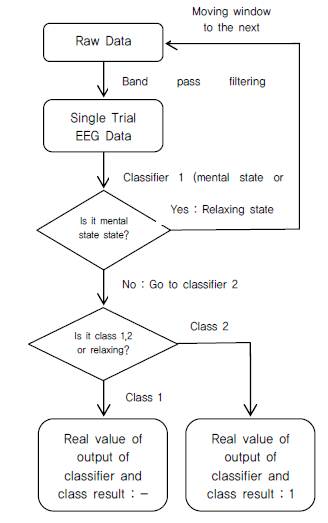
\includegraphics[width=4in]{method.png}
	%\renewcommand{\thefigure}{\arabic{figure}}
	\caption{ Working procedure }
	\label{Fig diagram}  
\end{figure}							
\section{Preprocessing}
\justify In this step the data is processed for the classifier to be trained and tested. Brain signals are generally very noisy and they contain some additional information that hampers the classifier's classification ability. Also the maximum portion of desired information can be found in a certain band of frequency, So it is imperative that the signals are processed before being feed in to the classifier.
\justify They are descried below.
\subsection{Data Extraction}
\justify In this step we have applied here are class selection, channel selection and bandpass filter application to keep only the classes, channels and frequency band we need rather than taking all the available data. This results in less redundant dataset.

\subsubsection{Bandpass Filter Application}
\justify Applying the bandpass filter is almost an essential part of classifying any kind of EEG data as certain information about certain task are mostly found in certain frequency bands.
\justify In out background study we have found that mostly two bandpass filters have been used while working with the dataset 1 of the BCI Competition IV, Butterworth and Chebychev. We have selected Butterworth filters.
\justify In the case of selecting frequency band When passing the data through the bandpass filter, we have found that the frequency band 4 hz to 35 hz shows in the better accuracy in all the cases.
\subsection{Feature Extraction}
\justify In the EEG data collected from the scalp there are different types of frequency components that gets added to the electrical signal of the brain. But more importantly we don't necessarily need al the components. With feature selection we try to get the frequency components that are more dominant in all the data and that has better correlation to the output.
\justify In this work, we have decided to use the Common spatial pattern(CSP) as the feature extraction method. the user can decide how many features are to be extracted from the data. it can be as many as the number of 59 channels to 1 .
\subsection{Feature Selection}
\justify After feature extraction, the process of selecting the best features among the extracted feature set is called feature selection. It it used to reduce the dimensionality of the data and train the data with only the best features. Thus improving the accuracy and training time.
\justify The feature selection method we have used is the SelectKBest method. This method chooses the features in the dataset that contributes most to the label or the target variable. The user can choose the number features to keep and it must be less then the number of extracted features.
\section{Classification}
\justify In this step after the data has been preprocessed and the features has been extracted, the feature set is to be trained and tested. But which classification algorithm is to be implemented is based on user's choice. Sequentially all the selected classification algorithm is implemented and the preprocessed data is used to train and test the classification model.

\subsection{Support-Vector Machine (SVM)}
\justify Support-vector machines (SVMs) are a type of supervised learning models and associated algorithms used for classification and regression analysis in machine learning. They work by creating a hyperplane in a high-dimensional space that separates the input data into two or more categories. SVMs are particularly useful for binary classification problems where the goal is to separate data into two classes.

The hyperplane is chosen such that it maximizes the distance between the two nearest data points of different classes. This distance is known as the margin, and the SVM algorithm seeks to find the hyperplane with the largest margin.

The decision boundary of an SVM can be expressed mathematically as:

\begin{equation}
	f(x) = \text{sign}(\vec{w} \cdot \vec{x} - b)
\end{equation}

where $\vec{w}$ is the weight vector that defines the hyperplane, $\vec{x}$ is the input data point, $b$ is the bias term, and $\text{sign}$ is the sign function that maps the output of the dot product to the positive or negative class. The weight vector and bias term are learned from the training data using an optimization algorithm such as gradient descent.

SVMs can also perform non-linear classification by using a kernel function to transform the input data into a higher-dimensional space where it can be linearly separated. The kernel function is chosen based on the characteristics of the input data and can be a polynomial, Gaussian, or other function.

\justify Various variations of SVM are available, which are created by using different kernels. Here we have used three of those variations.
\begin{itemize}
	\item SVM using Linear kernel
	\item SVM using Polynomial kernel
	\item SVM using Gaussian radial basis function(RBF) kernel
\end{itemize}


\section{Result Representation}
\justify The result here refers to the performances of the classification algorithms as well as used preprocessing methods. This performance is usually measured in various matrices. The metrics we have used are accuracy and kappa score.
\subsection{Accuracy}
\justify
When we refer to accuracy in the context of classification, we are typically talking about classification accuracy. This metric represents the proportion of correctly classified samples to the total number of input samples. However, it is important to note that classification accuracy is reliable only if there is an equal number of samples in each class.
\begin{equation}
	Accuracy = \frac{Number\; of\;correct\; predictions}{Number\;of\;total\; predictions\;made}
\end{equation}
\subsection{Kappa Value}
\justify Kappa value is a statistical coefficient that is used to measure inter-rater reliability for categorical items\cite{48}. The use of the kappa statistic is often preferred over simple percent agreement calculation since it considers the likelihood of the agreement happening by chance, making it a more reliable measure.
\begin{equation}
	k= 1- \frac{1 -  the\;relative\;observed\;agreement\;among\;raters}{1 - the\; hypothetical\;probability\;of\;chance\;agreement }
\end{equation} 
\subsection{Confusion Matrix}
\justify Confusion Matrix is a performance measurement for machine learning classification. Confusion matrix, also known as an error matrix\cite{50_10}, is a specific table layout that allows visualization of the performance of an algorithm, typically a supervised learning one (in unsupervised learning it is usually called a matching matrix). Each row of the matrix represents the instances in a predicted class, while each column represents the instances in an actual class\cite{49_11}.
\begin{figure}[t]
	
	
	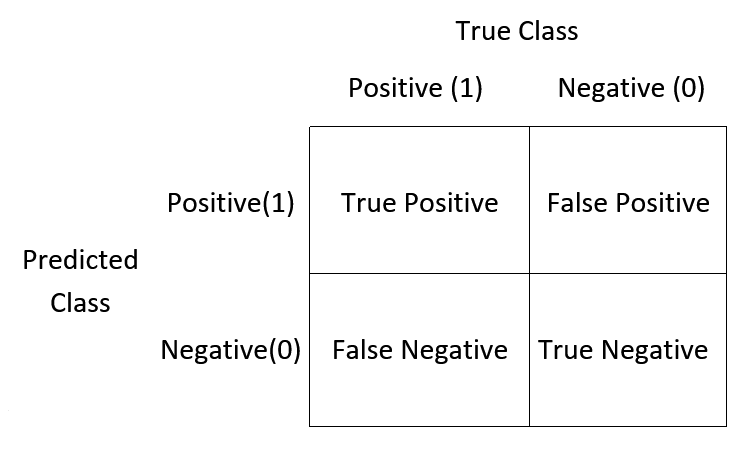
\includegraphics[width=\textwidth]{conf_matrix_t.png}
	%\renewcommand{\thefigure}{\arabic{figure}}
	\caption{ Confusion matrix for binary classification}
	\label{cnf_matrix_t}
\end{figure}

\newpage
	\chapter{ANALYSIS}
	\rule{14.6cm}{.05cm}
	\section{Introduction}
	\justify Analysis is the next stage of of our development process. This section must be completed before commencing the design of the software. This section will examine existing user practices to gain vital understanding of the business processes before undertaking a full requirements analysis that aims to define the systems functional architecture in terms of the operations or events that must be performed in order to achieve the project aim. Also, in this section existing alternative systems will be analyzed and their limitations taken into consideration during design and implementation.
	\section{Why do system fail?}
	\justify System development projects can fail for numerous reasons. A common cause of failure is a lack of resources allocated to researching and understanding the problem. Understanding the problem should include sufficient liaising with users and stakeholders of the system, but often IT developers neglect this vital communication, thus fail to accurately understand the business needs of the stakeholder and inaccurately define project objectives. User involvement throughout the requirements, design and implementation stage is therefore essential.
	\section{Software Requirements}
The objectives for this project are:
\begin{enumerate}
	\item Research existing technologies available.
	\item Research and choose a development methodology to follow
	\item Study various available datasets for continuous EEG data .
	\item Study various fast and efficient preprocessing, feature extraction and selection techniques and choose some for implementation.
	\item study and train machine learning models using the selected dataset to identify the MI task on real time.
	\item study and train machine learning models that can classify the identified MI task on real time. 
	\item Evaluate the application in terms of accuracy, effectiveness and meeting the requirements.
\end{enumerate}

	
	
	\newpage
	
%	\chapter{DESIGN}
%	\rule{14.6cm}{.05cm}

	\chapter{IMPLEMENTATION}
	\rule{14.6cm}{.05cm}
	\section{Introduction}
	\justify The implementation phase of the project is the development of the designs produced during the design phase Through a series of screen shots, code snippets and descriptions this section will show how we are trying to meet the generic requirements of the application, and where necessary the differences between the proposed designs and actual implementation.
	%\section{Data stores}
	%	\subsection{MATLAB Array}
	\section{Implementation Methodology}
	\justify  The GUI is built using the tkinter library and provides buttons for importing a dataset and classifying the motor imagery in the dataset. The GUI also displays the video frames corresponding to the classified motor imagery.
	
	\justify In this project defines a class GUI that inherits from tk.Tk. The \_\_init\_\_ method initializes the GUI window and creates the various widgets (import button, label and textbox for file path, play button, and canvas to display video frames). The import\_file method opens a file dialog to select a dataset file and displays the file path in the textbox. The play\_video method loads the dataset and applies a bandpass filter to the signal. It then applies feature engineering and classification using two trained classifiers to classify the motor imagery in the dataset. The method then loads the appropriate video and displays the video frames in the canvas.
	
	\justify The classifiers in this code are machine learning models that are trained on a dataset of EEG signals corresponding to motor imagery tasks. The classifiers are used to predict the class of a given EEG signal, either left hand or right hand motor imagery.
	
	\justify The EEG signals are first preprocessed by applying a bandpass filter to extract the relevant frequency components (4-35 Hz). Then, feature engineering is performed using Common Spatial Patterns (CSP) and SelectKBest feature selection methods. These features are fed into the classifiers, which use the learned patterns to predict the class of the EEG signal.
	
	\justify In this specific implementation, two classifiers are used in a cascade approach. If the first classifier predicts that the EEG signal corresponds to no motor imagery task, the second classifier is not called. Otherwise, the signal is passed to the second classifier, which makes the final prediction.
	\section{Interface and results}
	\justify As stated in chapters 2, good usability is critical to a successful solution to my end users problem. This design was chosen and implemented because of its clear layout and navigation structure. The final interface can be viewed in \ref{Fig main_ui}.
	
	\begin{figure}[b]
		\centering 
		
		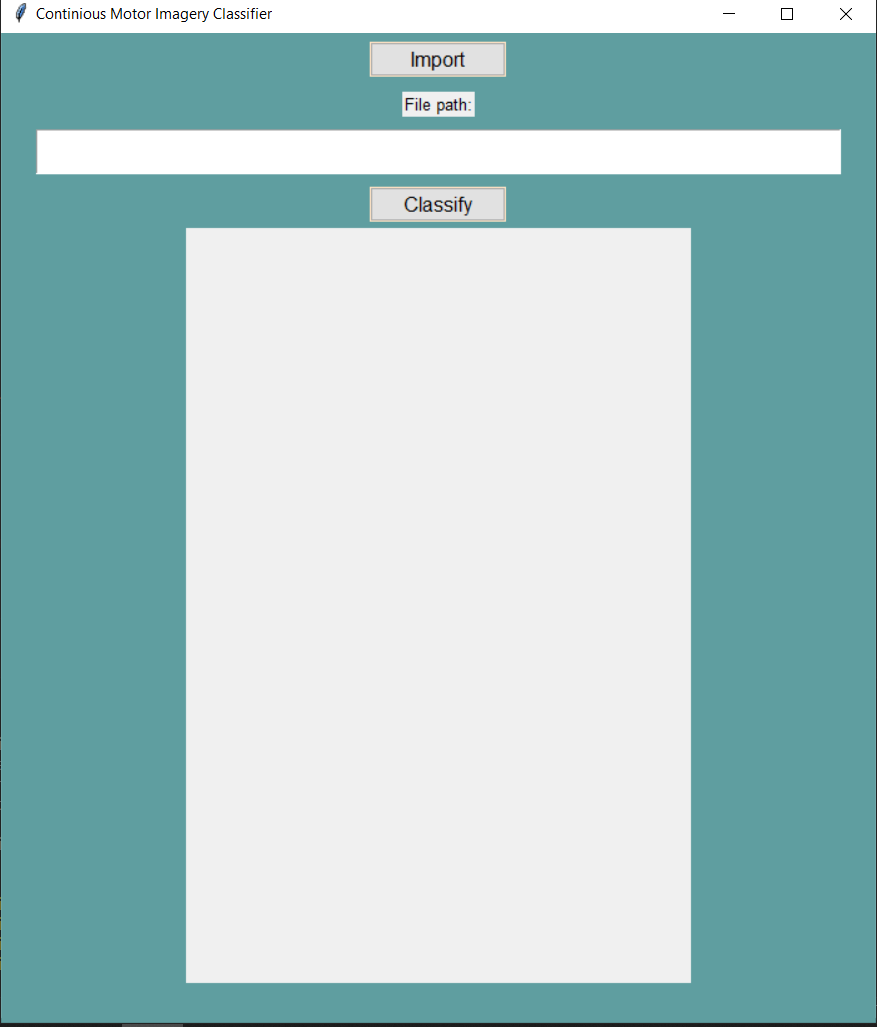
\includegraphics[height =4in]{1 (5).PNG}
		%\renewcommand{\thefigure}{\arabic{figure}}
		\caption{ The screenshot of final UI}
		\label{Fig main_ui}
	\end{figure}
	\justify \ref{Fig import} show what the ui will show during dataset import
\begin{figure}[h]
	\centering 
	
	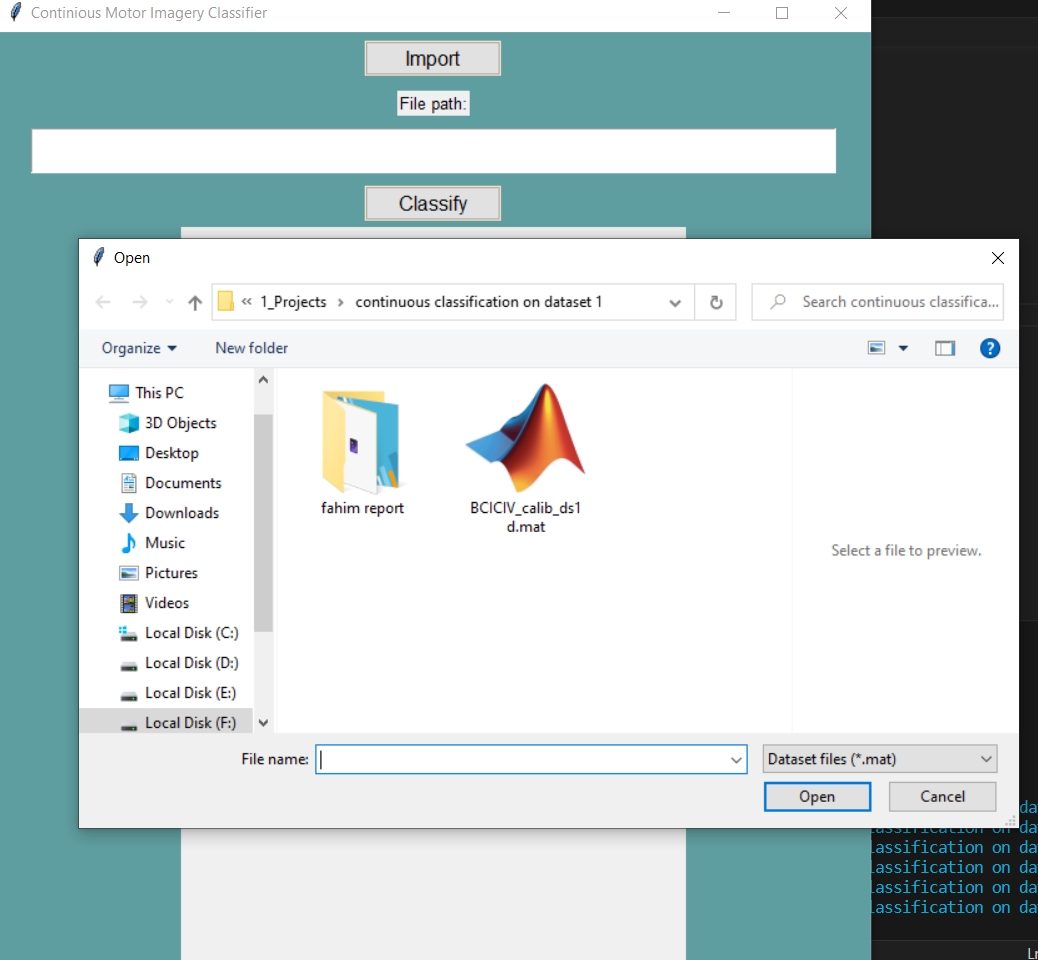
\includegraphics[height =4in]{1 (3).PNG}
	%\renewcommand{\thefigure}{\arabic{figure}}
	\caption{ The screenshot of importing dataset}
	\label{Fig import}
\end{figure}
\justify \ref{Fig after import} show what the ui will show after the dataset has been imported and ready for classification.
\begin{figure}[h]
	\centering 
	
	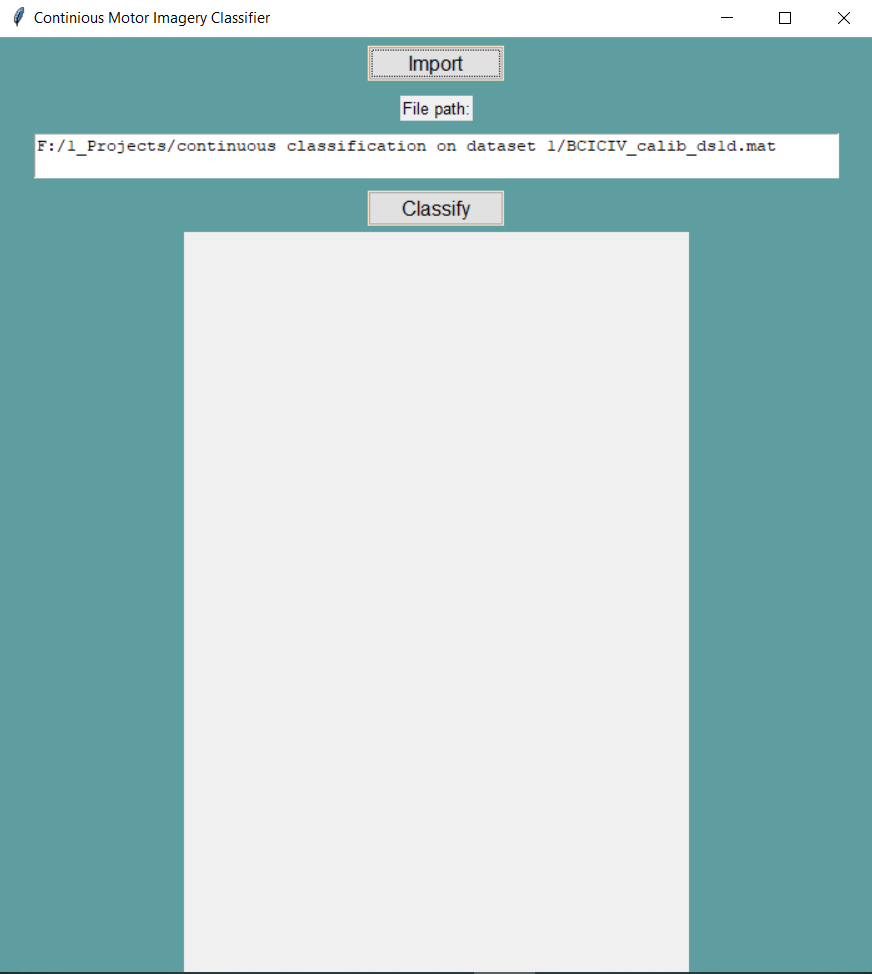
\includegraphics[height =4in]{1 (2).PNG}
	%\renewcommand{\thefigure}{\arabic{figure}}
	\caption{ The screenshot of state of UI after importing dataset}
	\label{Fig after import}
\end{figure}
	\justify \ref{Fig wave_left} show what the ui will show if the output of the classification is left hand
		\begin{figure}[h]
		\centering 
		
		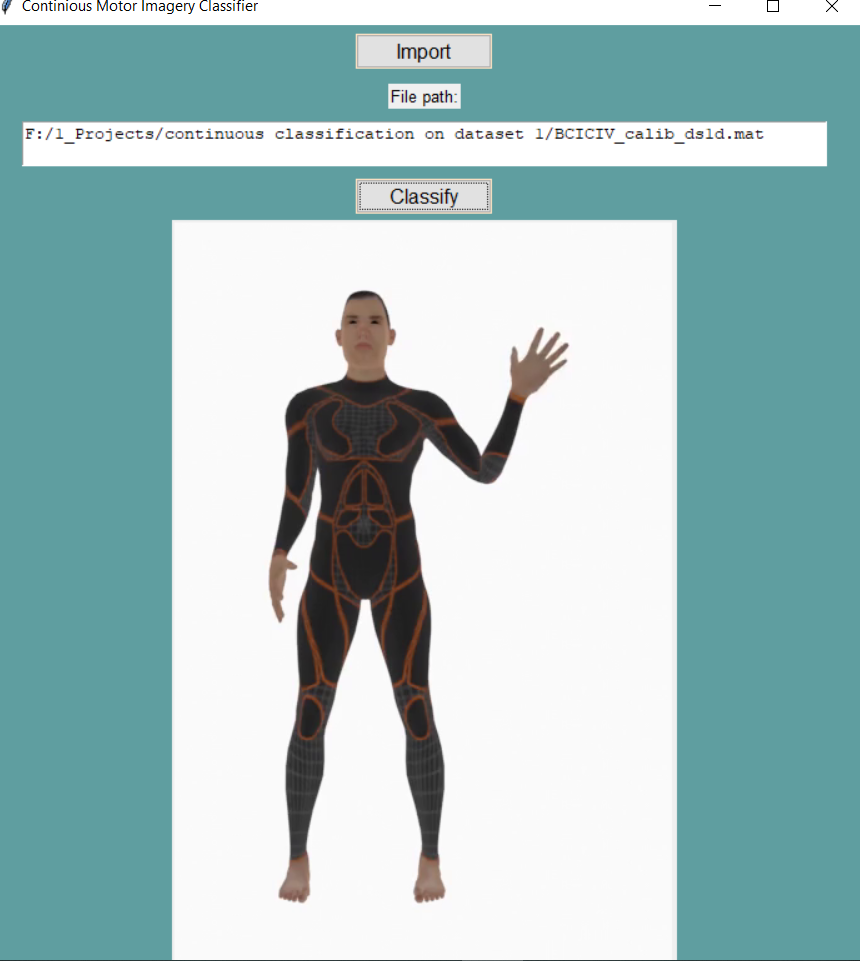
\includegraphics[height =4in]{1 (4).PNG}
		%\renewcommand{\thefigure}{\arabic{figure}}
		\caption{ The screenshot of final UI waving left hand}
		\label{Fig wave_left}
		\end{figure}
\justify \ref{Fig wave_right} show what the ui will show if the output of the classification is right hand.
		\begin{figure}[h]
	\centering 
	
	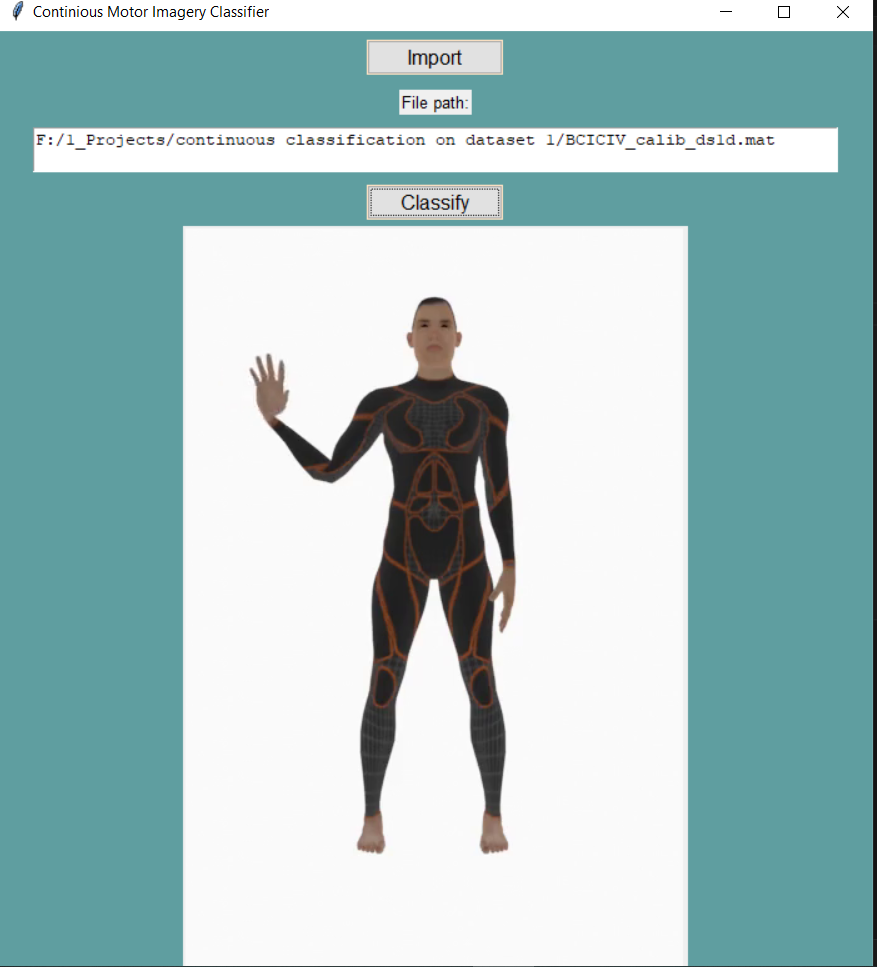
\includegraphics[height =4in]{1 (6).PNG}
	%\renewcommand{\thefigure}{\arabic{figure}}
	\caption{ The screenshot of final UI waving right hand}
	\label{Fig wave_right}
	\end{figure}
	%\subsection{Layout}
\justify \ref{Fig mi_nomi} show the Confusion matrix of MI/noMI classifier.

	\begin{figure}[h]
	\centering 
	
	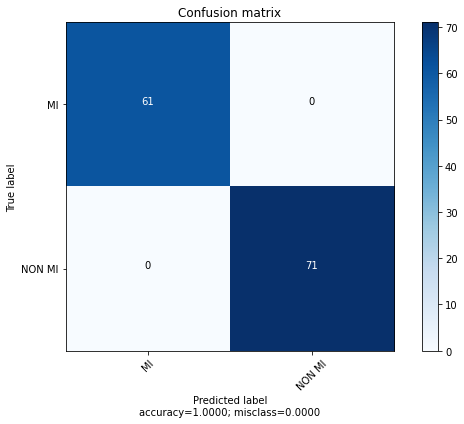
\includegraphics[height =4in]{cf1.png}
	%\renewcommand{\thefigure}{\arabic{figure}}
	\caption{ The screen shot of final UI}
	\label{Fig mi_nomi}
	\end{figure}
\justify \ref{Fig mi_nomi} show the Confusion matrix of MI classifier.	
		\begin{figure}[h]
		\centering 
		
		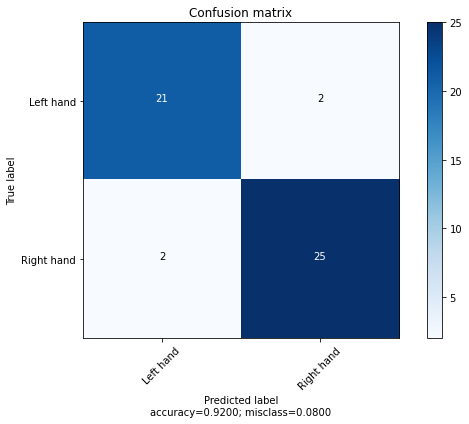
\includegraphics[height =4in]{cf2.png}
		%\renewcommand{\thefigure}{\arabic{figure}}
		\caption{ Confusion matrix of MI classifier}
		\label{Fig MI}
	\end{figure}
	

	\chapter{CONCLUSION}
	\rule{14.6cm}{.05cm}
	\section{Evaluation Of Entire Project}
	\justify In this project, our main objective was to build a system that could accurately classify different motor imagery tasks from a continuous stream of EEG data. We achieved this by utilizing various tools and techniques, including MATLAB, Python, and machine learning algorithms.
	
	\justify The dataset we used for this project consisted of EEG signals recorded from healthy subjects while they performed motor imagery tasks without feedback. For each subject, two classes of motor imagery were selected from the three classes of left hand, right hand, and foot, with the side chosen by the participant, optionally including both feet.
	
	\justify In the first two runs of the experiment, visual cues in the form of arrows pointing left, right, or down were presented on a computer screen. These cues were displayed for a period of 4 seconds during which the subject was instructed to perform the cued motor imagery task. These periods were interleaved with 2 seconds of a blank screen and 2 seconds with a fixation cross shown in the center of the screen. The fixation cross was superimposed on the cues, resulting in a 6-second duration.
	
	\justify The dataset we worked with contained continuous signals of 59 EEG channels and markers indicating the time points of cue presentation and the corresponding target classes. We used MATLAB to preprocess and convert the signals into uV values, and then used Python and machine learning algorithms to classify the different motor imagery tasks.
	
	\justify We found that Python was particularly useful for machine learning tasks, as it supports object-oriented, functional, and procedure-oriented styles of programming. We also utilized various packages in Python, including NumPy, SciPy, and scikit-learn, to implement our machine learning algorithms.
	
	\justify Overall, our system was able to correctly classify all motor imagery tasks from the continuous stream of EEG data with a high degree of accuracy. This has important implications for the development of brain-computer interfaces, which could potentially be used to help individuals with motor impairments to control devices and communicate more effectively.
	\section{Future Work}
	\justify As for future work, there are several avenues that can be explored to further improve the performance and usability of the system.
	
	\justify Firstly, more advanced machine learning algorithms can be used to improve the classification accuracy of the system. Deep learning models, such as convolutional neural networks (CNNs) or recurrent neural networks (RNNs), have shown promising results in the field of EEG-based motor imagery classification and could be integrated into the current system.
	
	\justify Secondly, the system can be extended to support real-time classification of motor imagery tasks. This would require optimizing the system for low-latency processing and developing a user-friendly interface for real-time feedback.
	
	\justify Thirdly, the system can be evaluated on a larger and more diverse dataset to assess its generalizability and robustness. This could involve collecting EEG data from a larger number of subjects with a wider range of demographics and motor imagery tasks.
	
	\justify Finally, the system can be integrated into a complete BCI system, which would allow users to control external devices using their brain signals. This would involve designing and implementing a user interface for device control and testing the system in a real-world setting.
	
	\justify Overall, there is still much room for improvement and innovation in the field of EEG-based motor imagery classification, and this project provides a solid foundation for future research and development.
	%\appendix

	\bibliography{citation}
	%\bibliographystyle{unsrt}
\bibliographystyle{IEEEtran}
\end{document}